Despite the many positive effects that game and gamification elements can have on their users, with the wrong type or the wrong amount of game mechanics implemented in the application, it can turn unmotivating or even frustrating.

A lot of games and gamified applications use leaderboards or other form of competition with either strangers, friends or both to motivate the user and increase replay value, creating incentives for the user to log on again the next day. While this might seem like an effective way to create engagement, the downside can be a forced sense of social obligations. The user might feel pressured to go online and do their daily challenges to not fall behind on the leaderboard, or feel peer pressure to partake in recurring events with their friends \cite{mmo}, potentially even making the user feel threatened if the competition with others is mandatory, especially if said competition is with co-workers or friends and family \cite{lifelong}. A good example of the use of leaderboards in a gamified context is the language learning application Duolingo (developed by Duolingo Inc., 2012), see Figure \ref{fig:1} \cite{leaderboard}. In the worst case this can create a dynamic like any other forced routine in day to day life, playing the game or using the app starts feeling like work or a chore, which either will cause unnecessary stress or will cause the user to stop using it eventually \cite{mmo}.

\begin{figure}[h]
    \centering
    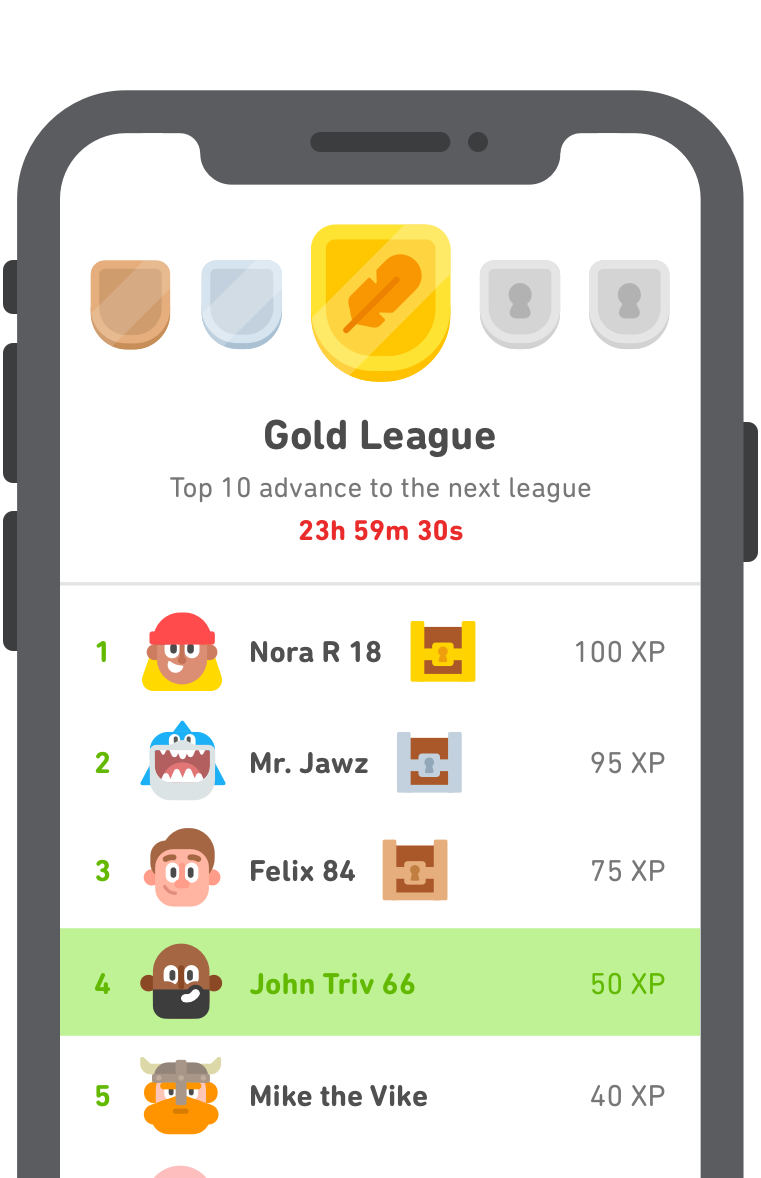
\includegraphics[width=0.48\textwidth]{figures/leaderboard}
    \caption{Leaderboard in Duolingo}
    \label{fig:1}
\end{figure}

Even without the social aspect, there might be systems in place that aim to motivate the user to come back, but trigger stress and negative reactions instead. Commonly, log-in streaks are used to reward the player for their commitment, but some applications dish out penalties instead if a day is missed, creating yet another cycle of frustration for the player. Once again, a good example of this is the application Duolingo which aims to motivate their users to return through a streak system, as can be seen on Figure \ref{fig:2} \cite{streak}.

\begin{figure}[h]
    \centering
    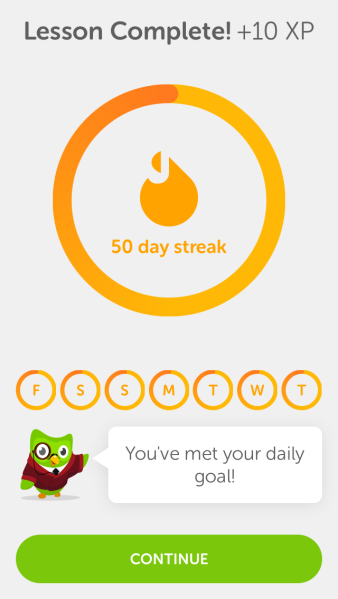
\includegraphics[width=0.46\textwidth]{figures/streak}
    \caption{Streak System in Duolingo}
    \label{fig:2}
\end{figure}

Well designed reward systems are powerful tools that are used within games or gamification to create a sense of success and progress, motivating and engaging the user or even inducing a state of flow, but not always do they trigger these feelings, instead promoting negative reactions if used improperly \cite{equilibrium}.

Shallow gamification heavily relies on extrinsic rewards to motivate their users instead of working on triggering the users intrinsic motivation, most notably through systems like points and badges. This may initially create engagement, using immediate gratification to keep the experience fun and stimulating, but it fails to maintain this engagement, making the user lack the necessary long-term investment in the activity that it takes for habits to be formed and goals to be achieved \cite{equilibrium}.
The reason why excessive use of extrinsic rewards hamper especially the users own intrinsic motivation can be explained by the paradox of the 'Overjustification Effect'. It has been observed that initially motivated individuals, which then recieve extrinsic rewards for the activity they have been doing previously, lose interest in this activity when those rewards cease to be given. The motivation for participation shifts from inherent enjoyment of the activity to the expectation for the next external reward, overshadowing any previously existing intrinsic motivation. The sole reason to keep partaking in the activity becomes the hunt for the next dopamine kick that the reward triggers \cite{equilibrium}.

The excessive use of rewards in gamified contexts also can come across as controlling, causing the user to feel less competent and like they are not in charge of their own process, equally decreasing intrinsic motivation.

While reward systems are an important part of making gamification work, using them too generously is more likely to backfire than to actually help the user to stay engaged. This seems to be commonly disregarded in the development of current gamified applications and might be why those gamification tools are failing today \cite{equilibrium}.